\documentclass[border=1cm]{standalone}
\usepackage{tikz}

\begin{document}

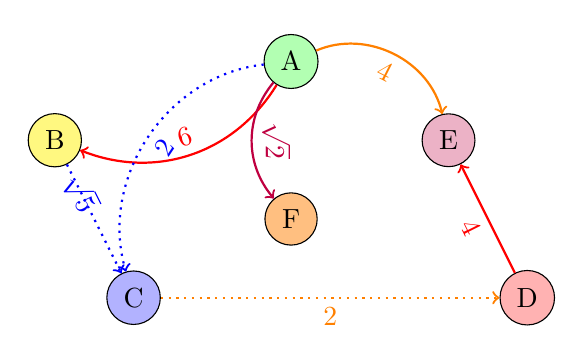
\begin{tikzpicture}


  \node[circle, draw, fill=green!30] (A) at (0, 2) {A};  
  \node[circle, draw, fill=yellow!50] (B) at (-3, 1) {B};   
  \node[circle, draw, fill=blue!30] (C) at (-2, -1) {C};   
  \node[circle, draw, fill=red!30] (D) at (3, -1) {D};   
  \node[circle, draw, fill=purple!30] (E) at (2, 1) {E};  
  \node[circle, draw, fill=orange!50] (F) at (0, 0) {F};  

  
  \draw[->, red, thick] (A) to[bend left=40] node[midway, above, sloped] {6} (B);  
  \draw[->, blue, dotted, thick] (A) to[bend right=50] node[midway, below, sloped] {2} (C);  
  \draw[->, orange, thick] (A) to[bend left=50] node[midway, below, sloped] {4} (E);  
  \draw[->, purple, thick] (A) to[bend right=40] node[midway, above, sloped] {$\sqrt{2}$} (F);  
  \draw[->, blue, dotted, thick] (B) -- (C) node[midway, left, sloped] {$\sqrt{5}$};  
  \draw[->, orange, dotted, thick] (C) -- (D) node[midway, below, sloped] {2};  
  \draw[->, red, thick] (D) -- (E) node[midway, below, sloped] {4};  

\end{tikzpicture}

\end{document}
\documentclass[border=1cm]{standalone}
\usepackage{tikz}
\usepackage{amsmath}

\begin{document}
\begin{tikzpicture}[scale=2]
